\appendices
\raggedbottom

\section{Pipeline Details} \label{app:pipeline}
\begin{figure}[H]
  \centering
  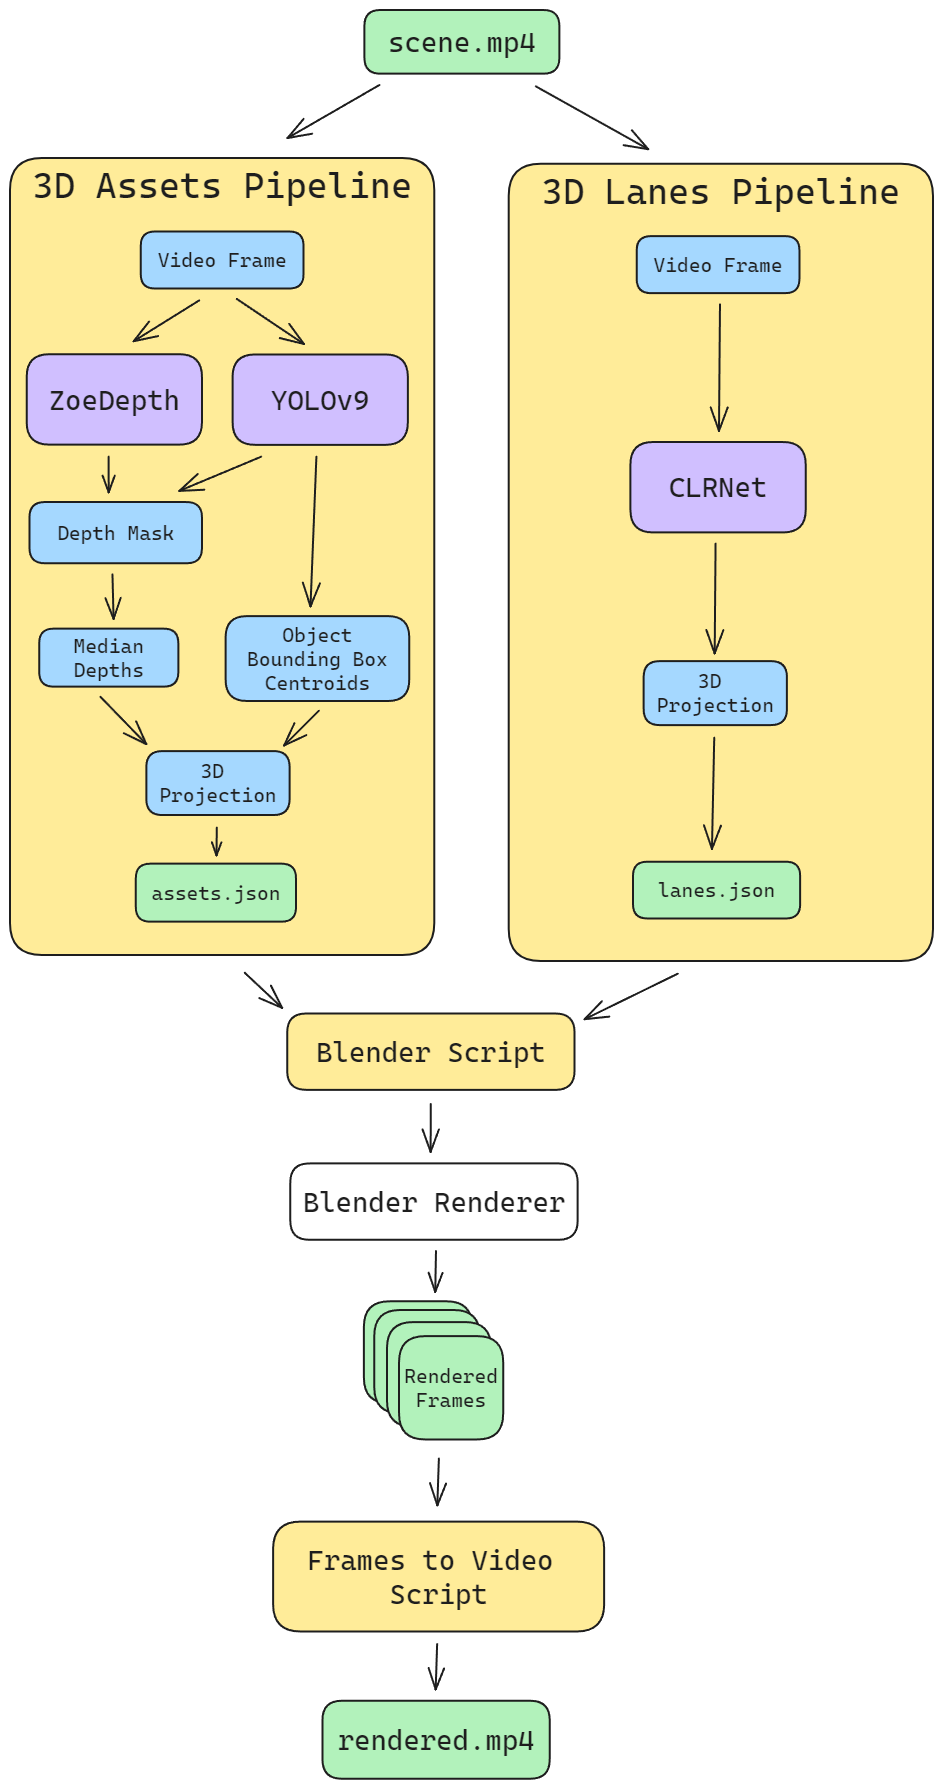
\includegraphics[width=0.95\linewidth]{images/pipeline.png}
  \caption{Final rendering pipeline. Green blocks are files, yellow blocks are Python scripts. Within the Python blocks, purple blocks are networks, and blue blocks are hand written steps.}
  \label{fig:pipeline}
\end{figure}

\newpage
\section{Results}\label{app:results}

\begin{figure}[H]
  \centering
  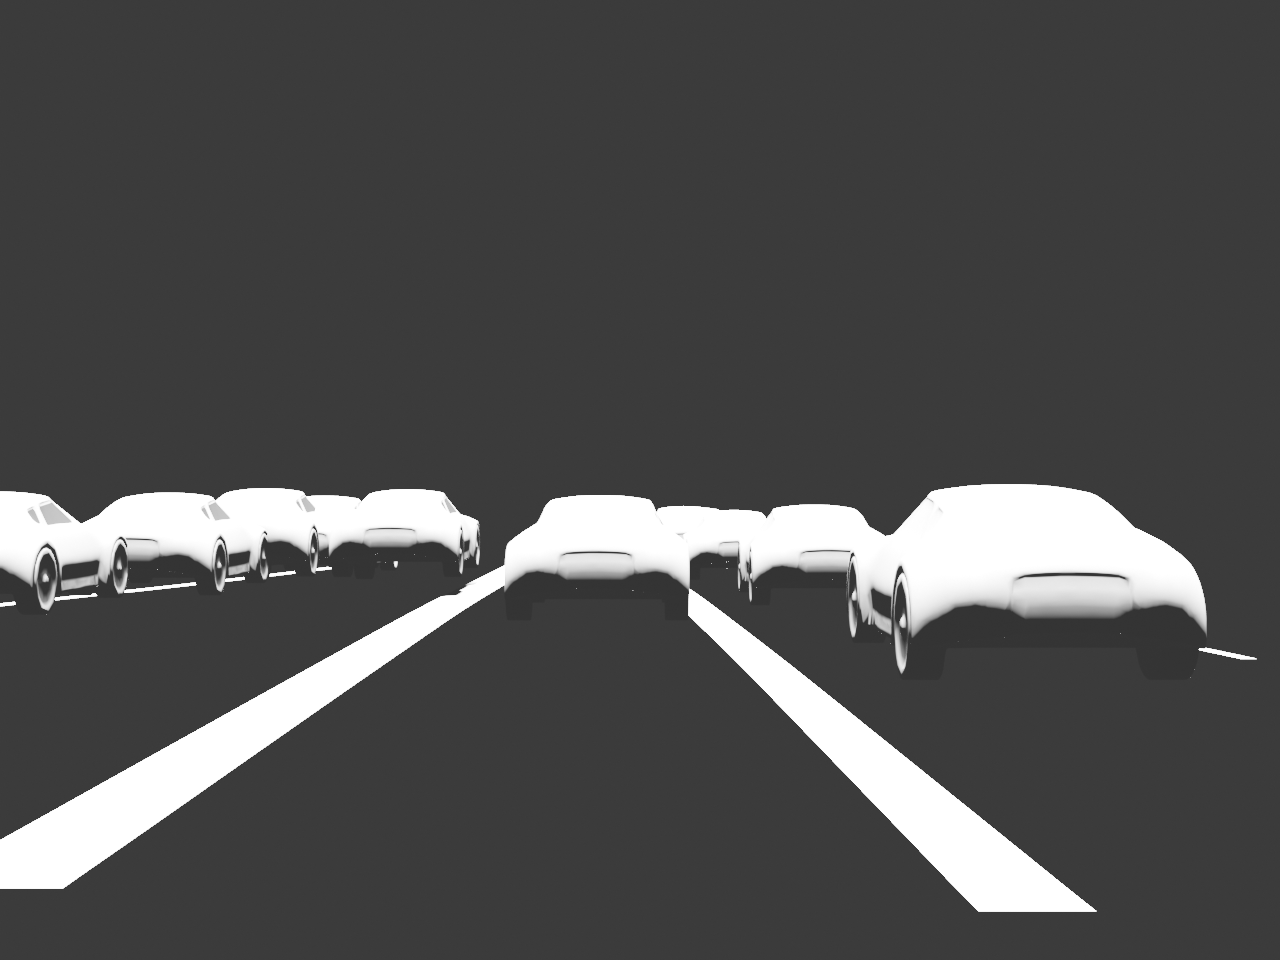
\includegraphics[width=0.95\linewidth]{images/results/scene6_943.png}
  \caption{Scene 6 output at frame 943.}
\end{figure}
\begin{figure}[H]
  \centering
  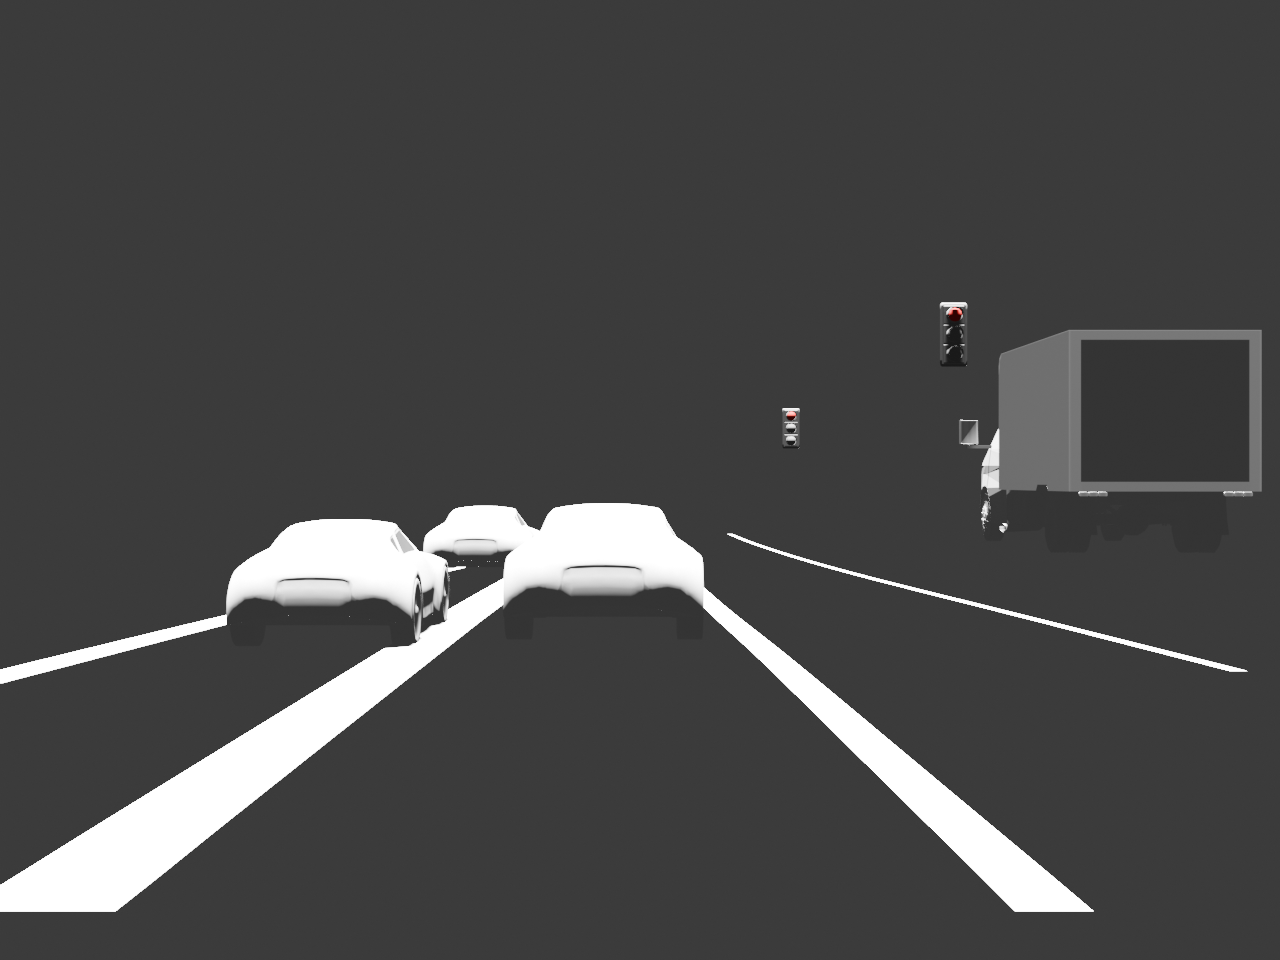
\includegraphics[width=0.95\linewidth]{images/results/scene7_frame583.png}
  \caption{Scene 7 output at frame 583.}
\end{figure}
\begin{figure}[H]
  \centering
  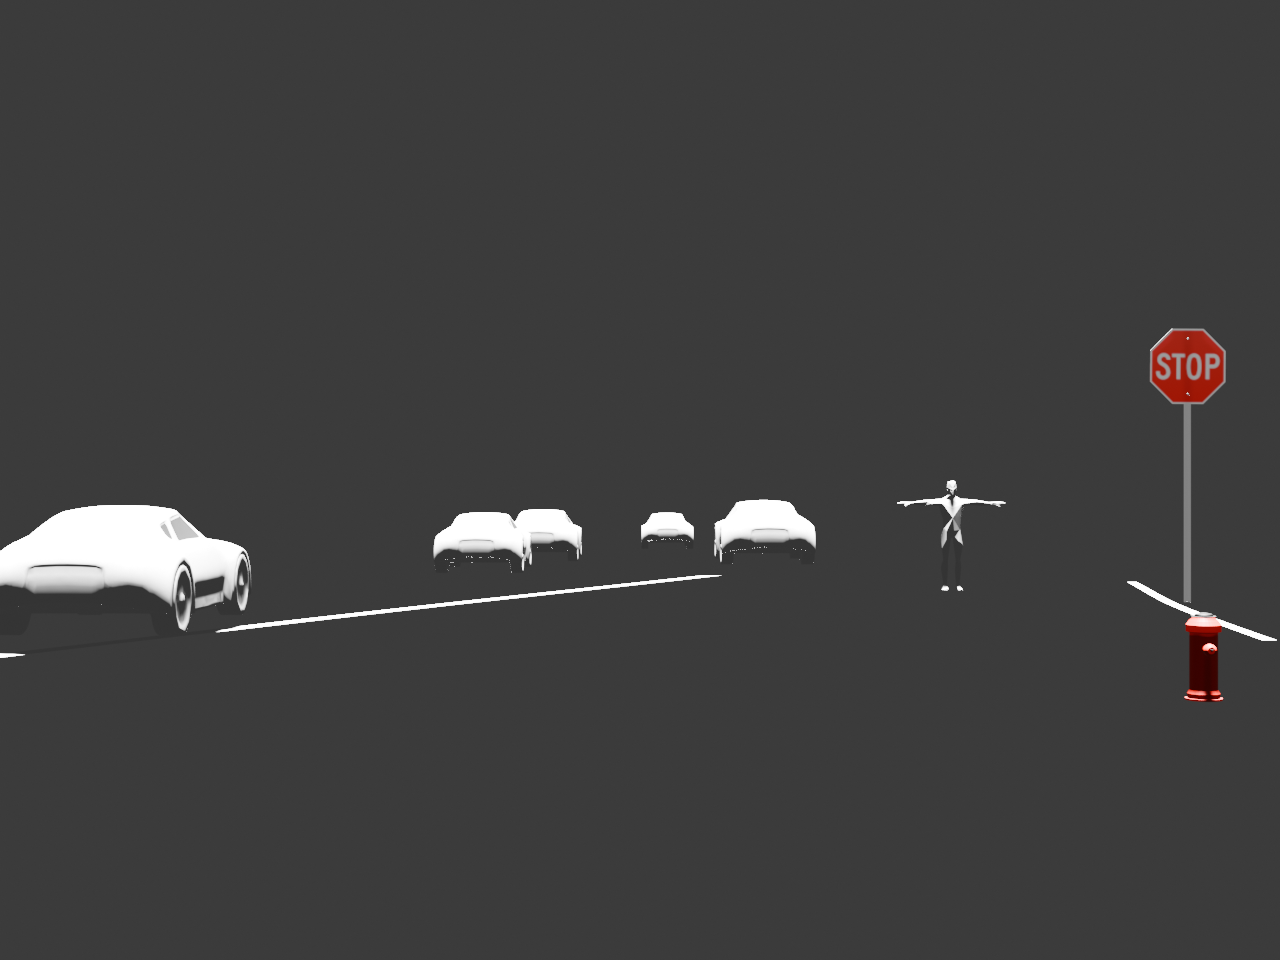
\includegraphics[width=0.95\linewidth]{images/results/scene8_frame547.png}
  \caption{Scene 8 output at frame 547.}
\end{figure}

\begin{figure}[H]
  \centering
  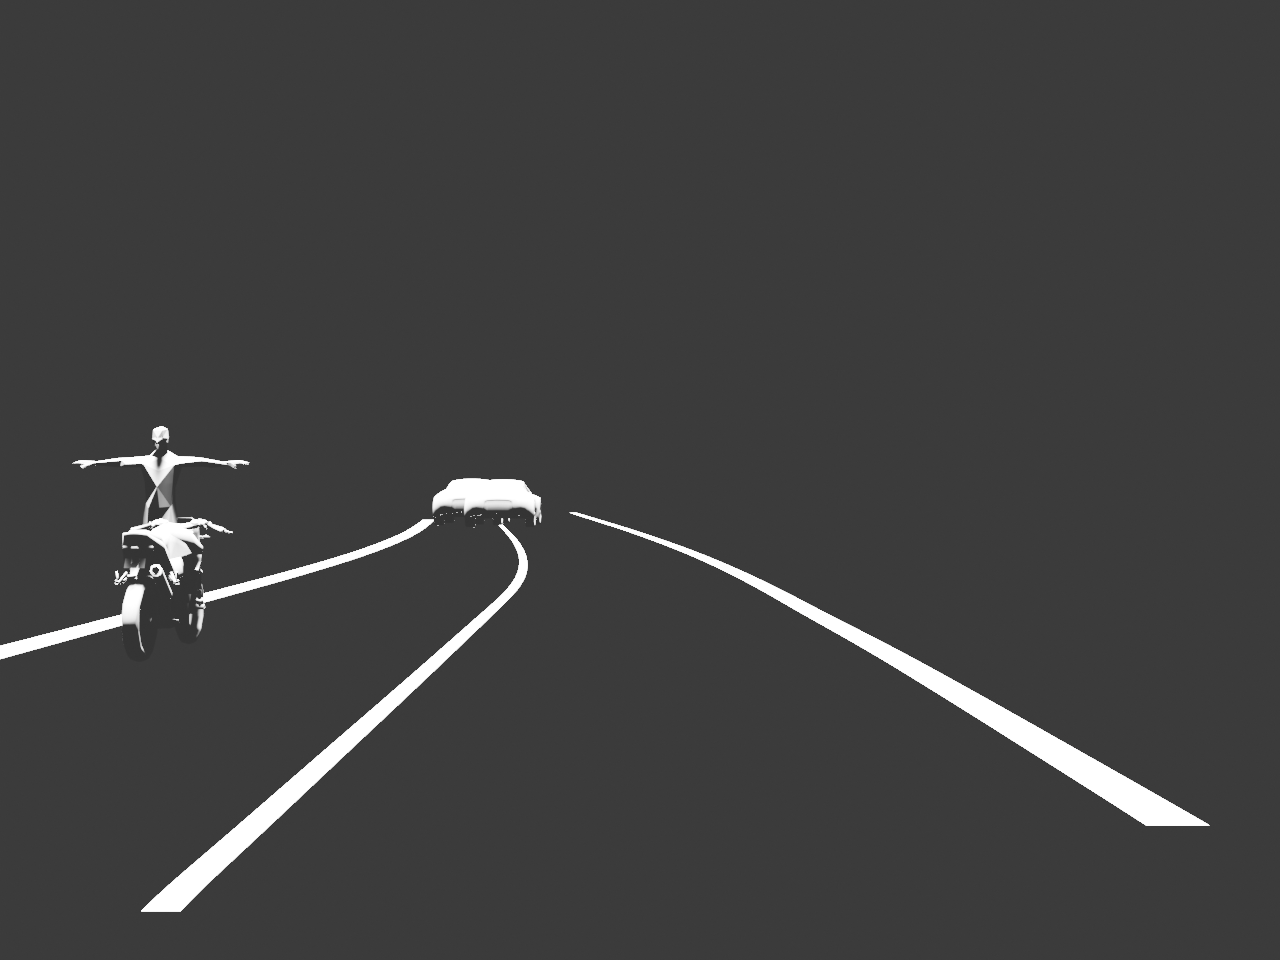
\includegraphics[width=0.95\linewidth]{images/results/scene13_frame1165.png}
  \caption{Scene 13 output at frame 1165.}
\end{figure}